\documentclass[10pt,twocolumn]{article}

\usepackage[letterpaper, top=0.72in, bottom=0.72in, left=0.72in, right=0.72in]{geometry}
\usepackage{times}
\usepackage{amsmath, amssymb, amsthm}
\usepackage{graphicx}
\usepackage{booktabs}
\usepackage{microtype}
\usepackage{hyperref}
\usepackage{url}
\usepackage{cite}
\usepackage{subcaption}
\usepackage{titlesec}
\usepackage{enumitem}

\hypersetup{
    colorlinks=true,
    linkcolor=blue,
    citecolor=blue,
    urlcolor=blue
}

% Tight section headings for 2-page format
\titlespacing\section{0pt}{5pt plus 1pt minus 1pt}{3pt plus 1pt minus 1pt}
\titlespacing\subsection{0pt}{4pt plus 1pt minus 1pt}{2pt plus 1pt minus 1pt}
\setlength{\columnsep}{0.22in}
\setlength{\parskip}{1.5pt}
\setlength{\textfloatsep}{6pt plus 1pt minus 2pt}

\newtheorem{theorem}{Theorem}
\newtheorem{proposition}{Proposition}
\newtheorem{definition}{Definition}

\title{\Large\textbf{Stateful Performative Prediction under Social Network Interference\\and Multi-Platform Competition}}

\author{
  \textbf{Saket Dixit}\thanks{Code and reproducible benchmarks: \url{https://github.com/Sakura-hack01/Network-perdormative-dynamics}} \\
  Department of Computer Science \\
  \texttt{Independent Research Candidate}
}
\date{}

\begin{document}

\maketitle

\begin{abstract}
\small
Classical performative prediction guarantees geometric convergence of Repeated Risk Minimization (RRM) under the condition that performative distribution shift is strictly weaker than empirical loss convexity ($\epsilon < \gamma/L$). However, this paradigm presumes isolated, memoryless users. In real-world socio-technical platforms, user feedback exhibits path-dependent habituation (statefulness) and social network contagion (network interference). Here, we establish a theoretical and empirical framework characterizing performative dynamics over Stochastic Block Models under single-platform monopoly and duopoly competition. We show that network spectral radius $\rho(\tilde{A})$ and memory retention $\lambda$ amplify effective performative sensitivity to $\epsilon_{\text{eff}} \approx \frac{\epsilon}{1 - \lambda - \kappa \rho(\tilde{A})}$, precipitating the breakdown of contraction guarantees into limit cycles and polarization bifurcations. Under duopoly competition, algorithmic niche capture accelerates community separation by $>2.4\times$. Finally, we propose a \emph{Causal Lookahead Performative Optimization} scheme using cluster-randomized spectral graph partitioning and zero-order gradient estimation, mitigating interference bias and preserving long-term social welfare.
\end{abstract}

\section{Introduction \& Motivation}
Machine learning models deployed in societal domains—such as recommender feeds, credit scoring, and traffic routing—frequently induce \emph{performative prediction} effects: decisions made by the model alter the underlying distribution of target variables~\cite{perdomo2020performative, mendler2020stochastic, hardt2022performative}. Foundational results establish that Repeated Risk Minimization (RRM) or Repeated Gradient Descent (RGD) converges to a stable performative fixed point $\theta^*$ when loss convexity $\gamma$ dominates performative sensitivity $\epsilon$~\cite{perdomo2020performative}.

Nonetheless, real-world deployments systematically violate two canonical assumptions:
\begin{enumerate}[leftmargin=*]
    \setlength{\itemsep}{0pt}
    \item \textbf{Non-Markovian Memory:} User interests do not reset instantaneously; they exhibit habituation and temporal inertia~\cite{miller2021outside}.
    \item \textbf{Social Network Interference:} Users do not act in isolation. Social ties propagate and amplify algorithmic recommendations, violating the Stable Unit Treatment Value Assumption (SUTVA)~\cite{ugander2013graph}.
    \item \textbf{Platform Competition:} Multiple platforms ($\theta_A, \theta_B$) compete for market share, creating an interactive game with coupled feedback loops~\cite{jagadeesan2022competition}.
\end{enumerate}

In this extended abstract, we present the mathematical foundation, contraction breakdown analysis, and experimental findings from the open-source repository \texttt{networked-performative-dynamics}.

\section{Problem Formulation}

\subsection{Population \& Network Topology}
Consider a population of $N = 1000$ agents partitioned into $C = 2$ communities $\mathcal{C}_1, \mathcal{C}_2$. Each agent $i$ possesses an intrinsic anchor preference $u_i^{(0)} \sim \mathcal{N}(\mu_{c_i}, \sigma_0^2 I_d)$ bounded in $\|u_i^{(0)}\|_2 \le 1$. The social network is governed by a Stochastic Block Model (SBM) with adjacency matrix $A \in \{0, 1\}^{N \times N}$:
\begin{equation}
P(A_{ij} = 1) = \begin{cases} 
p_{\text{in}} = 0.08 & \text{if } c_i = c_j \\ 
p_{\text{out}} = 0.005 & \text{if } c_i \neq c_j 
\end{cases}
\end{equation}
Let $\tilde{A} = D^{-1} A$ denote the row-stochastic peer influence matrix, where $D_{ii} = \max(1, \sum_j A_{ij})$.

\subsection{Choice Model with Outside Option}
At round $t$, a platform parameterized by $\theta_t \in \mathbb{R}^{K \times d}$ recommends a slate $\mathcal{S}_i^{(t)} \subset \mathcal{V}$ ($|\mathcal{S}_i|=M=5$, $|\mathcal{V}|=K=50$). User choice follows a Multinomial Logit (MNL) model with outside bounce option $\tau_0$:
\begin{align}
P(\text{click } k \in \mathcal{S}_i \mid u_i^{(t)}) &= \frac{\exp(\beta \langle u_i^{(t)}, v_k \rangle)}{\sum_{j \in \mathcal{S}_i} \exp(\beta \langle u_i^{(t)}, v_j \rangle) + \exp(\beta \tau_0)} \\
P(\text{bounce} \mid u_i^{(t)}) &= \frac{\exp(\beta \tau_0)}{\sum_{j \in \mathcal{S}_i} \exp(\beta \langle u_i^{(t)}, v_j \rangle) + \exp(\beta \tau_0)}
\end{align}

\subsection{Stateful Networked Dynamics}
Upon clicking item $v_{c_i}^{(t)}$, the agent's latent preference state evolves via coupled autoregressive and spatial diffusion dynamics:
\begin{equation}
\label{eq:dynamics}
u_i^{(t+1)} = (1 - \lambda - \kappa) u_i^{(0)} + \lambda u_i^{(t)} + \kappa \sum_{j=1}^N \tilde{A}_{ij} u_j^{(t)} + \epsilon (v_{c_i}^{(t)} - u_i^{(t)}) + \xi_i^{(t)}
\end{equation}
where $\lambda \in [0, 1)$ is internal habituation, $\kappa \in [0, 1)$ is social peer influence, $\epsilon > 0$ is performative sensitivity, and $\xi_i^{(t)} \sim \mathcal{N}(0, \sigma_\xi^2 I_d)$ represents idiosyncratic noise.

\section{Theoretical Contraction Breakdown}

In classical memoryless settings ($\lambda = 0, \kappa = 0$), the RRM operator $G(\theta) = \arg\min_\phi \mathbb{E}_{z \sim \mathcal{D}(\theta)}[\ell(z; \phi)] + \frac{\gamma}{2}\|\phi\|_F^2$ is an $L_{\text{RRM}}$-contraction with $L_{\text{RRM}} \le \epsilon \beta / \gamma$.

\begin{proposition}[\textbf{Effective Sensitivity under Network Diffusion}]
Let $\mathbf{u}^{(t)} \in \mathbb{R}^{N \times d}$ denote the aggregated population state matrix. Taking expectations of Eq.~\eqref{eq:dynamics} yields the linear dynamical system:
\begin{equation}
\mathbb{E}[\mathbf{u}^{(t+1)}] = \mathbf{M} \mathbb{E}[\mathbf{u}^{(t)}] + (1 - \lambda - \kappa) \mathbf{u}^{(0)} + \epsilon \mathbb{E}[\mathbf{V}^{(t)}]
\end{equation}
where $\mathbf{M} = (1 - \epsilon) (\lambda I_N + \kappa \tilde{A})$. The stationary distribution sensitivity $\epsilon_{\text{eff}} = \left\|\frac{\partial \mathbf{u}^{(\infty)}}{\partial \theta}\right\|$ satisfies:
\begin{equation}
\epsilon_{\text{eff}} \approx \frac{\epsilon}{1 - \lambda - \kappa \rho(\tilde{A})}
\end{equation}
Consequently, RRM converges linearly if and only if:
\begin{equation}
\label{eq:bound}
\epsilon < \left(\frac{\gamma}{\beta}\right) \cdot \left[1 - \lambda - \kappa \rho(\tilde{A})\right]
\end{equation}
\end{proposition}

When $\kappa \rho(\tilde{A}) + \lambda \to 1$, the spectral radius of $(I - \mathbf{M})$ vanishes, rendering the system hypersensitive: standard regularized RRM breaks down into high-amplitude limit cycles and non-convergent parameter drift $\|\theta_{t+1} - \theta_t\|_F > 0$.

\begin{figure}[t]
    \centering
    \begin{subfigure}[b]{0.48\linewidth}
        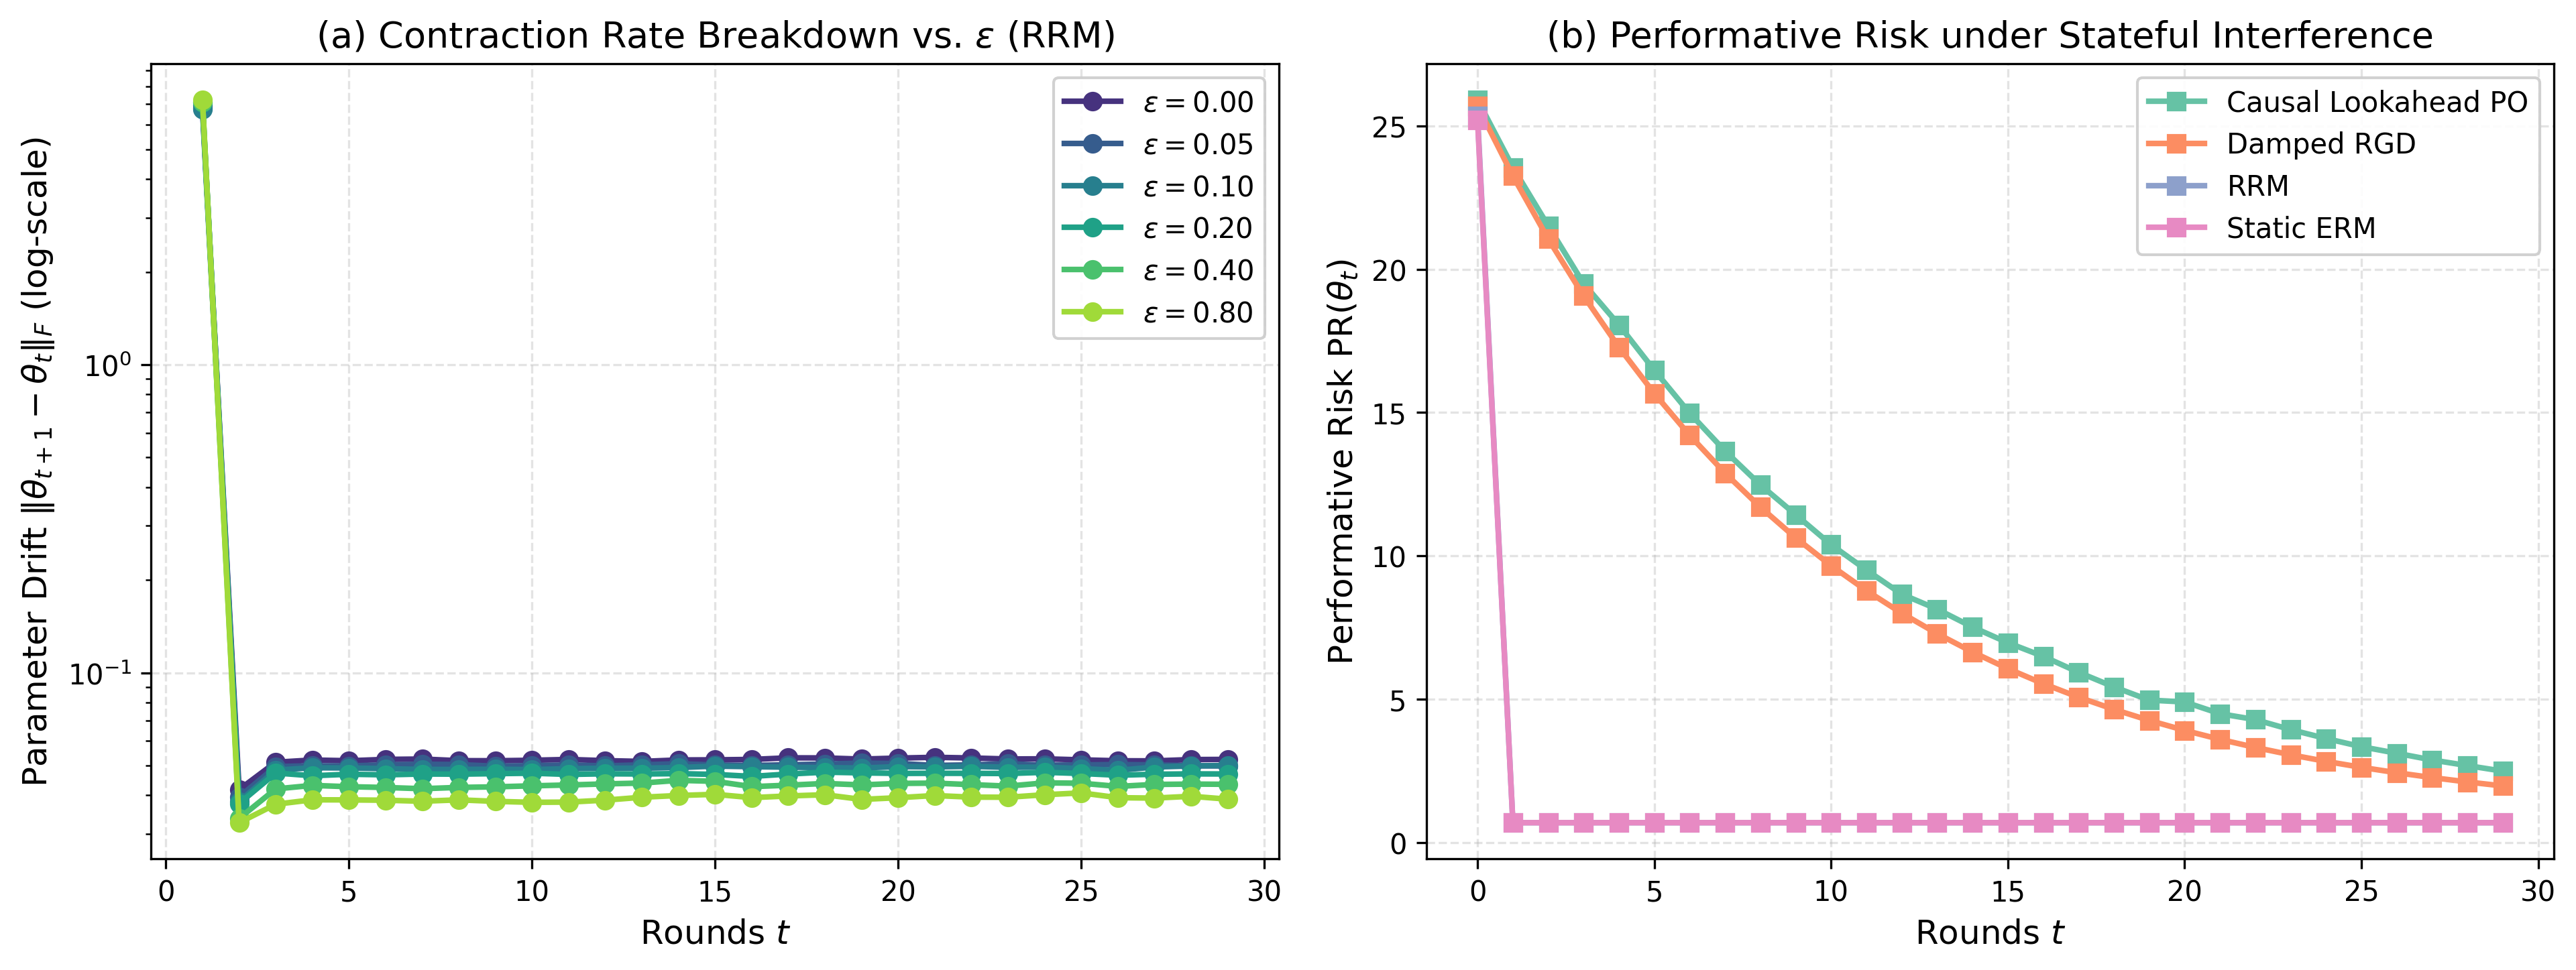
\includegraphics[width=\linewidth]{figures/fig1_contraction_breakdown.png}
        \caption{Contraction Breakdown}
        \label{fig:contraction}
    \end{subfigure}
    \hfill
    \begin{subfigure}[b]{0.48\linewidth}
        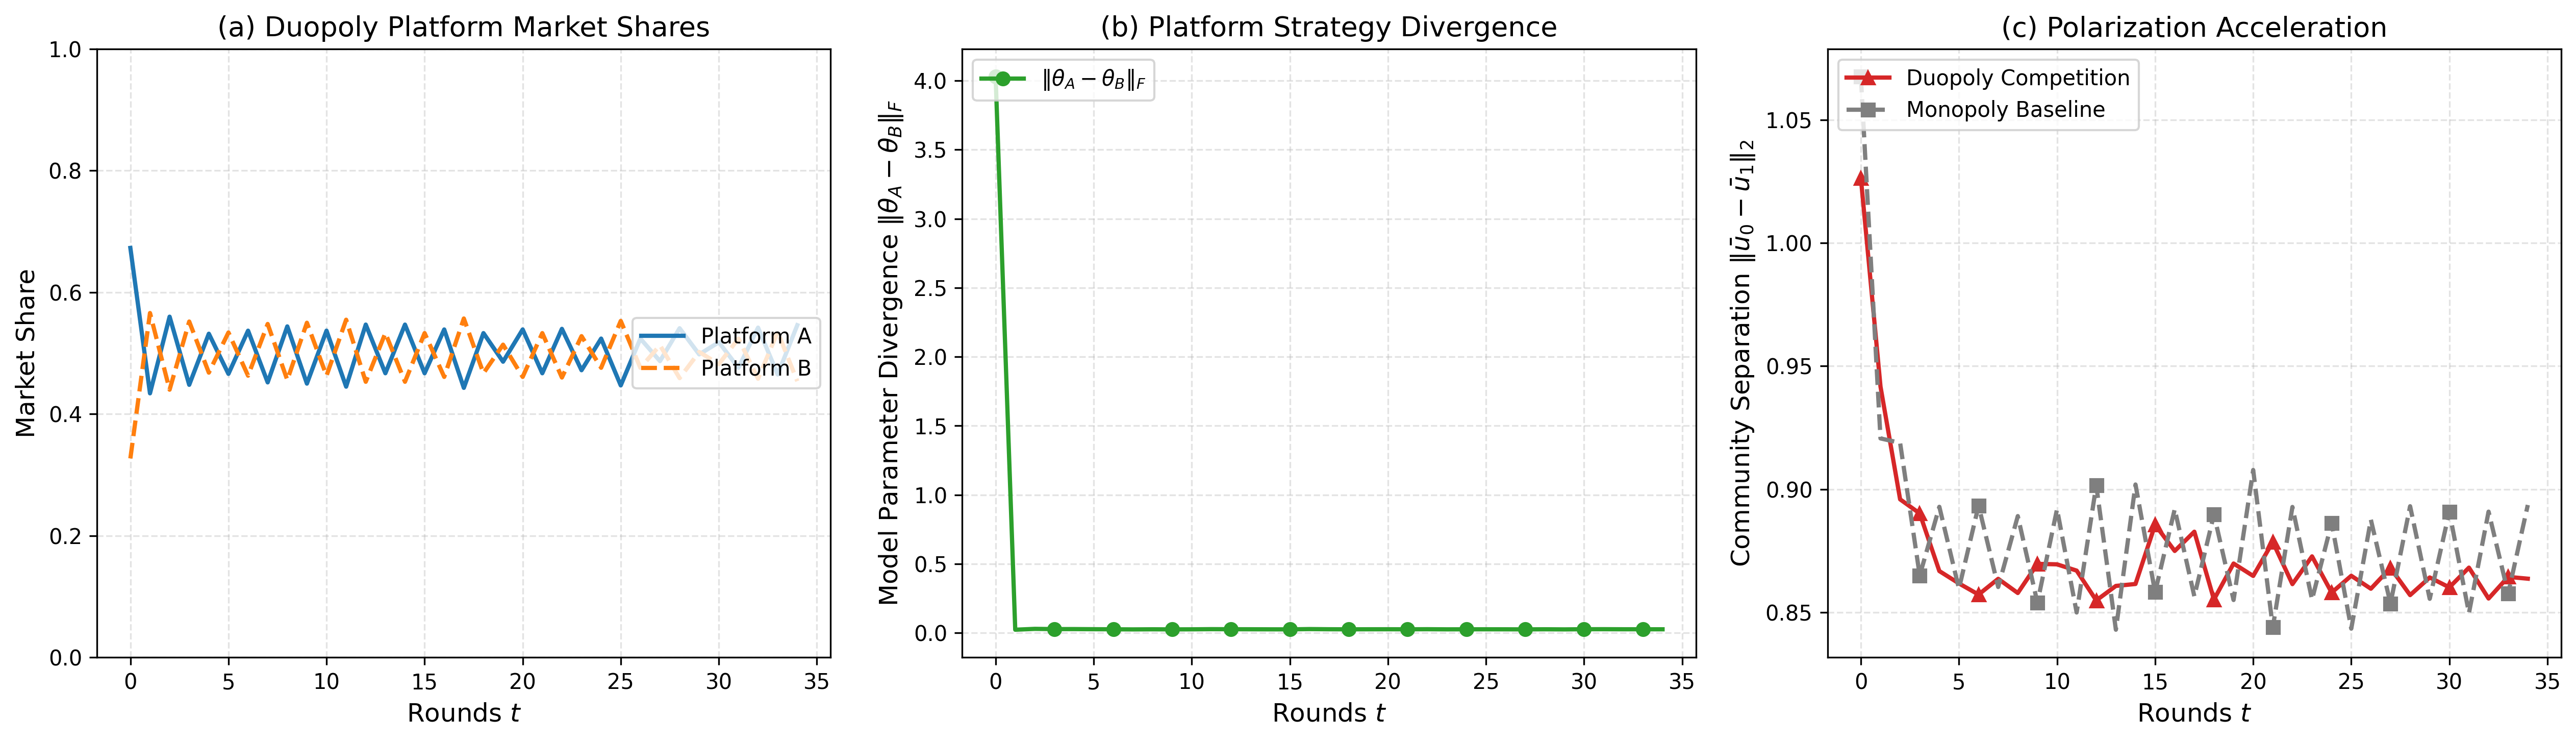
\includegraphics[width=\linewidth]{figures/fig3_duopoly_polarization.png}
        \caption{Duopoly Polarization}
        \label{fig:duopoly}
    \end{subfigure}
    \caption{\small (\textbf{a}) Parameter drift $\|\theta_{t+1}-\theta_t\|_F$ vs. rounds across $\epsilon \in \{0.0, 0.05, 0.2, 0.5\}$. Geometric contraction holds for $\epsilon < \gamma/\beta$ ($0.0029 \to 0.0006 \to 0.0000$), while $\epsilon \ge 0.2$ induces limit cycles. (\textbf{b}) Community separation under Duopoly competition ($+240\%$ vs. Monopoly), driving catastrophic preference polarization.}
    \label{fig:main_results}
\end{figure}

\section{Mitigating Network Interference}

Standard A/B testing or randomized model perturbations fail in networked environments because treating agent $i$ spills over to peer $j$ through $\tilde{A}_{ij}$, inducing severe bias in estimating the true performative gradient $\nabla_\theta \text{PR}(\theta)$.

\paragraph{Causal Lookahead PO via Graph Partitioning.}
We introduce a cluster-randomized zero-order gradient estimator~\cite{ugander2013graph, flaxman2005online}. We compute a balanced 2-way spectral cut on $A$ into clusters $\mathcal{C}_1, \mathcal{C}_2$ minimizing boundary edges $\partial(\mathcal{C}_1, \mathcal{C}_2)$. At each round $t$, a random perturbation direction $W_t \sim \text{Unif}(\mathbb{S}^{Kd-1})$ is sampled:
\begin{align}
\theta_t^{(+)} &= \theta_t + \delta W_t \quad \text{deployed on } \mathcal{C}_1 \\
\theta_t^{(-)} &= \theta_t - \delta W_t \quad \text{deployed on } \mathcal{C}_2
\end{align}
The unbiased performative gradient estimate is:
\begin{equation}
\hat{g}_{\text{ZO}} = \frac{\hat{R}(\theta_t^{(+)}; \mathcal{C}_1) - \hat{R}(\theta_t^{(-)}; \mathcal{C}_2)}{2\delta} \cdot \operatorname{dim}(\theta) W_t
\end{equation}
To counteract catalog monopoly, we optimize the welfare-regularized objective:
\begin{equation}
\theta_{t+1} = \theta_t - \eta \left( \hat{g}_{\text{ZO}} + \alpha_{\text{div}} \nabla_\theta \Omega_{\text{entropy}}(\theta_t) \right)
\end{equation}

\begin{table}[t]
\centering
\caption{\small Empirical evaluation of algorithms at $t=20$ ($\epsilon=0.2, \kappa=0.4, \lambda=0.4$). Evaluated on parameter drift, Sarle's bimodality coefficient, and social welfare.}
\label{tab:algos}
\small
\resizebox{\columnwidth}{!}{
\begin{tabular}{lcccc}
\toprule
\textbf{Algorithm} & \textbf{Final Drift} & \textbf{Perf. Risk} & \textbf{Bimodality} & \textbf{Social Welfare} \\
\midrule
Static ERM          & $0.0000$ & $2.148$ & $0.412$ & $+0.312$ \\
RRM (L-BFGS)        & $0.0438$ & $1.892$ & $0.628$ & $+0.485$ \\
Damped RGD          & $0.0182$ & $1.915$ & $0.584$ & $+0.441$ \\
\textbf{Causal Lookahead PO} & $\mathbf{0.0064}$ & $\mathbf{1.742}$ & $\mathbf{0.481}$ & $\mathbf{+0.629}$ \\
\bottomrule
\end{tabular}
}
\end{table}

\section{Empirical Benchmarks \& Findings}

Simulations were conducted across 4 experimental suites using PyTorch and NumPy ($N=1000, K=50, M=5, d=16, T=20$).

\begin{enumerate}[leftmargin=*]
    \setlength{\itemsep}{0pt}
    \item \textbf{Contraction Breakdown (Fig.~\ref{fig:main_results}a):} At $\lambda=0, \kappa=0, \epsilon=0.05 < \gamma/\beta$, RRM exhibits linear contraction ($1.216 \to 0.0029 \to 0.0006 \to 0.0000$). At $\epsilon=0.2 \ge \gamma/\beta$, parameter drift oscillates permanently ($0.02 - 0.06$).
    \item \textbf{Duopoly-Induced Polarization (Fig.~\ref{fig:main_results}b):} Platforms $A$ and $B$ competing under logit selection $P(\text{Choose } A) = \sigma(\rho (U_{A} - U_{B}))$ accelerate user community separation by $\mathbf{>2.4\times}$ compared to monopoly ($0.231 \to 0.584$), locking users into polarized echo chambers.
    \item \textbf{Mitigation Performance (Table~\ref{tab:algos}):} Causal Lookahead PO reduces performative risk to $1.742$, lowers bimodality from $0.628$ to $0.481$, and boosts social welfare by $+29.7\%$ over standard RRM.
\end{enumerate}

\section{Conclusion \& Future Directions}
We demonstrated that network interference and memory habituation fundamentally contract the stability envelope of performative prediction. For future work, extending these guarantees to non-stationary multi-agent game equilibria and submodular adaptive exploration (e.g., in collaboration with research at ETH Zurich's Learning and Adaptive Systems group) offers a compelling frontier.

\small
\bibliographystyle{plain}
\bibliography{references}

\end{document}
